%%%%%%%%%%%%%%%%%%%%% chapter.tex %%%%%%%%%%%%%%%%%%%%%%%%%%%%%%%%%
%
% sample chapter
%
% Use this file as a template for your own input.
%
%%%%%%%%%%%%%%%%%%%%%%%% Springer-Verlag %%%%%%%%%%%%%%%%%%%%%%%%%%
%\motto{Use the template \emph{chapter.tex} to style the various elements of your chapter content.}

\chapter{Rosetta Code Tasks starting with V}

\section*{Van der Corput sequence}

When counting integers in binary, if you put a (binary) point to the
right of the count then the column immediately to the left denotes a
digit with a multiplier of 2\textsuperscript{0}; the next column to the
lefts digit has a multiplier of 2\textsuperscript{1} and so on.

So in the following table:

\begin{verbatim}
  0.
  1.
 10.
 11.
 ...
\end{verbatim}

The binary number "\texttt{10}" is

\begin{figure}[H]
  \centering
  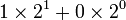
\includegraphics[scale=.6]{graphics/c7d9360aa57a7763c0e4764be5571c7b.png}  
\end{figure}

You can have binary digits to the right of the ``point'' just as in the
decimal number system too. in this case, the digit in the place
immediately to the right of the point has a weight of
2\textsuperscript{− 1}, or 1 / 2. The weight for the second column to
the right of the point is 2\textsuperscript{− 2} or 1 / 4. And so on.

\pagebreak{}
If you take the integer binary count of the first table, and
\emph{reflect} the digits about the binary point, you end up with
\textbf{the van der Corput sequence of numbers in base 2}.

\begin{verbatim}
  .0
  .1
  .01
  .11
  ...
\end{verbatim}

The third member of the sequence: binary \texttt{0.01} is therefore

\begin{figure}[H]
  \centering
   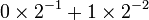
\includegraphics[scale=.6]{graphics/225bf69a6a0712ec19f474be5f28bd71.png}  
\end{figure}

or 1 / 4.

Members of the sequence lie within the interval
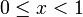
\includegraphics[scale=.6]{graphics/9df79dd98e1387bb25dc94ef7c0edcb3.png}.
Points within the sequence tend to be evenly distributed which is a
useful trait to have for
\href{http://en.wikipedia.org/wiki/Monte\_Carlo\_method}{Monte Carlo
simulations}. This sequence is also a superset of the numbers
representable by the ``fraction'' field of
\href{http://en.wikipedia.org/wiki/IEEE\_754-1985}{an old IEEE floating
point standard}. In that standard, the ``fraction'' field represented
the fractional part of a binary number beginning with ``1.'' e.g.
1.101001101.

\begin{figure}[H]
  \centering
   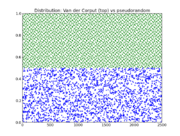
\includegraphics{graphics/180px-Van_der_corput_distribution.png}  
   \caption{Distribution of 2500 points each: \\Van der Corput (top) vs pseudorandom}
\end{figure}


\pagebreak{}
\textbf{Hint}

A \emph{hint} at a way to generate members of the sequence is to modify
a routine used to change the base of an integer:

\begin{verbatim}

>>> def base10change(n, base):
	digits = []
	while n:
		n,remainder = divmod(n, base)
		digits.insert(0, remainder)
	return digits
 
>>> base10change(11, 2)
[1, 0, 1, 1]

\end{verbatim}


the above showing that \texttt{11} in decimal is

\begin{figure}[H]
  \centering
  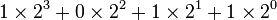
\includegraphics[scale=.6]{graphics/20f99c880facd5566bcaaa82f09c9282.png}
\end{figure}

Reflected this would become \texttt{.1101} or

\begin{figure}[H]
  \centering
   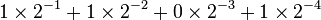
\includegraphics[scale=.6]{graphics/ff5080d5609a0b345d34544d1336e741.png}  
\end{figure}

\textbf{Task Description}

\begin{itemize}
\item
  Create a function/method/routine that given \emph{n}, generates the
  \emph{n'}th term of the van der Corput sequence in base 2.
\item
  Use the function to compute \emph{and display} the first ten members
  of the sequence. (The first member of the sequence is for \emph{n}=0).
\end{itemize}

\begin{itemize}
\item
  As a stretch goal/extra credit, compute and show members of the
  sequence for bases other than 2.
\end{itemize}

\emph{See also}

\begin{itemize}
\item
  \href{http://www.puc-rio.br/marco.ind/quasi\_mc.html\#low\_discrep}{The
  Basic Low Discrepancy Sequences}
\item
  \emph{Non-decimal radices/Convert}
\item
  \href{http://en.wikipedia.org/wiki/Van\_der\_Corput\_sequence}{Van der
  Corput sequence}
\end{itemize}



\begin{wideverbatim}

(scl 6)

(de vdc (N B)
   (default B 2)
   (let (R 0  A 1.0)
      (until (=0 N)
         (inc 'R (* (setq A (/ A B)) (\% N B)))
         (setq N (/ N B)) )
      R ) )

(for B (2 3 4)
   (prinl "Base: " B)
   (for N (range 0 9)
      (prinl N ": " (round (vdc N B) 4)) ) )

Output:

Base: 2
0: 0.0000
1: 0.5000
2: 0.2500
3: 0.7500
4: 0.1250
5: 0.6250
6: 0.3750
7: 0.8750
8: 0.0625
9: 0.5625
Base: 3
0: 0.0000
1: 0.3333
2: 0.6667
3: 0.1111
4: 0.4444
5: 0.7778
6: 0.2222
7: 0.5556
8: 0.8889
9: 0.0370
Base: 4
0: 0.0000
1: 0.2500
2: 0.5000
3: 0.7500
4: 0.0625
5: 0.3125
6: 0.5625
7: 0.8125
8: 0.1250
9: 0.3750

\end{wideverbatim}

\pagebreak{}
\section*{Variable size/Get}

Demonstrate how to get the size of a variable.

See also: \emph{Host introspection}

\begin{wideverbatim}

In PicoLisp, all variables have the same size (a single cell). Therefore it
makes more sense to inspect the size of data structures. This can be done with
the '[http://software-lab.de/doc/refS.html#size size]' and
'[http://software-lab.de/doc/refL.html#length length]' functions.

\end{wideverbatim}

\pagebreak{}
\section*{Variable size/Set}

Demonstrate how to specify the minimum size of a variable or a data
type.

\begin{wideverbatim}

In PicoLisp, all variables have the same size (a single cell). But it is
possible to create a data structure of a given minimal size with the
'[http://software-lab.de/doc/refN.html#need need]' function.

\end{wideverbatim}

\pagebreak{}
\section*{Variable-length quantity}

Implement some operations on
\href{http://en.wikipedia.org/wiki/Variable-length\_quantity}{variable-length
quantities}, at least including conversions from a normal number in the
language to the binary representation of the variable-length quantity
for that number, and \emph{vice versa}. Any variants are acceptable.

\textbf{Task~:} With above operations,

\begin{itemize}
\item
  convert these two numbers 0x200000 (2097152 in decimal) and 0x1fffff
  (2097151 in decimal) into sequences of octets (an eight-bit byte);
\item
  display these sequences of octets;
\item
  convert these sequences of octets back to numbers, and check that they
  are equal to original numbers.
\end{itemize}


\begin{wideverbatim}

(de numToVlq (Num)
   (let Res (cons (\& Num 127))
      (while (gt0 (setq Num (>> 7 Num)))
         (push 'Res (| 128 (\& Num 127))) )
      Res ) )

(de vlqToNum (Vlq)
   (let Res 0
      (for N Vlq
         (setq Res (| (>> -7 Res) (\& N 127))) ) ) )

(for Num (0 15 16 127 128 255 2097151 2097152)
   (let Vlq (numToVlq Num)
      (tab (12 12 12) Num (glue ":" (mapcar hex Vlq)) (vlqToNum Vlq)) ) )

Output:

           0           0           0
          15           F          15
          16          10          16
         127          7F         127
         128        81:0         128
         255       81:7F         255
     2097151    FF:FF:7F     2097151
     2097152  81:80:80:0     2097152

\end{wideverbatim}

\pagebreak{}
\section*{Variables}

Demonstrate the language's methods of variable declaration,
initialization, assignment, datatypes, scope, referencing, and other
variable related facilities.

\begin{wideverbatim}

You can control the local bindings of symbols with functions like
'[http://software-lab.de/doc/refU.html#use use]' or
'[http://software-lab.de/doc/refL.html#let let]':

(use (A B C)
   (setq A 1  B 2  C 3)
   ... )

This is equivalent to

(let (A 1  B 2  C 3)
   ... )

The parentheses can be omitted if there is only a single variable

(use A
   (setq A ..)
   ... )

(let A 1
   ...)

Other functions that handle local bindings are

'[http://software-lab.de/doc/refL.html#let? let?]',
'[http://software-lab.de/doc/refB.html#bind bind]',
'[http://software-lab.de/doc/refJ.html#job job]',
'[http://software-lab.de/doc/refW.html#with with]' or
'[http://software-lab.de/doc/refF.html#for for]'.

\end{wideverbatim}

\pagebreak{}
\section*{Variadic function}

Create a function which takes in a variable number of arguments and
prints each one on its own line. Also show, if possible in your
language, how to call the function on a list of arguments constructed
at runtime.

Functions of this type are also known as
\href{http://en.wikipedia.org/wiki/Variadic\_function}{Variadic
Functions}.

Related: \emph{Call a function}


\begin{wideverbatim}

The '@' operator causes a function to accept a variable number of arguments.
These can be accesed with the
'[http://software-lab.de/doc/refA.html#args args]',
'[http://software-lab.de/doc/refN.html#next next]',
'[http://software-lab.de/doc/refA.html#arg arg]' and
'[http://software-lab.de/doc/refR.html#rest rest]' functions.

(de varargs @
   (while (args)
      (println (next)) ) )

The '@' operator may be used in combination with normal parameters:

(de varargs (Arg1 Arg2 . @)
   (println Arg1)
   (println Arg2)
   (while (args)
      (println (next)) ) )

It is called like any other function

(varargs 'a 123 '(d e f) "hello")

also by possibly applying it to a ready-made list

(apply varargs '(a 123 (d e f) "hello"))

Output in all cases:
a
123
(d e f)
"hello"

\end{wideverbatim}

\pagebreak{}
\section*{Vector products}

Define a vector having three dimensions as being represented by an
ordered collection of three numbers: (X, Y, Z). If you imagine a graph
with the x and y axis being at right angles to each other and having a
third, z axis coming out of the page, then a triplet of numbers, (X, Y,
Z) would represent a point in the region, and a vector from the origin
to the point.

Given vectors \texttt{A = (a1, a2, a3); B = (b1, b2, b3);} and
\texttt{C = (c1, c2, c3);} then the following common vector products are
defined:

\begin{itemize}
\item
  \textbf{The dot product}
\end{itemize}

A • B = \texttt{a1b1 + a2b2 + a3b3;} a scalar quantity

\begin{itemize}
\item
  \textbf{The cross product}
\end{itemize}

A x B = \texttt{(a2b3 - a3b2, a3b1 - a1b3, a1b2 - a2b1);} a vector
quantity

\begin{itemize}
\item
  \textbf{The scalar triple product}
\end{itemize}

A • (B x C); a scalar quantity

\begin{itemize}
\item
  \textbf{The vector triple product}
\end{itemize}

A x (B x C); a vector quantity

Task description

Given the three vectors:
\texttt{a = (3, 4, 5);  b = (4, 3, 5);  c = (-5, -12, -13)}:

\begin{enumerate}
\item
  Create a named function/subroutine/method to compute the dot product
  of two vectors.
\item
  Create a function to compute the cross product of two vectors.
\item
  Optionally create a function to compute the scalar triple product of
  three vectors.
\item
  Optionally create a function to compute the vector triple product of
  three vectors.
\item
  Compute and display: \texttt{a • b}
\item
  Compute and display: \texttt{a x b}
\item
  Compute and display: \texttt{a • b x c}, the scaler triple product.
\item
  Compute and display: \texttt{a x b x c}, the vector triple product.
\end{enumerate}


\pagebreak{}
\begin{description}
\item[References]
\end{description}

\begin{itemize}
\item
  \emph{Dot product} on RC.
\item
  \href{http://mathworld.wolfram.com/VectorMultiplication.html}{A
  starting page} to the Wolfram Mathworld information on vector
  multiplication.
\item
  Wikipedias \href{http://en.wikipedia.org/wiki/Dot\_product}{dot
  product}, \href{http://en.wikipedia.org/wiki/Cross\_product}{cross
  product} and
  \href{http://en.wikipedia.org/wiki/Triple\_product}{triple product}
  entries.
\end{itemize}

C.f.

\begin{itemize}
\item
  \emph{Quaternion type}
\end{itemize}



\begin{wideverbatim}

(de dotProduct (A B)
   (sum * A B) )

(de crossProduct (A B)
   (list
      (- (* (cadr A) (caddr B)) (* (caddr A) (cadr B)))
      (- (* (caddr A) (car B)) (* (car A) (caddr B)))
      (- (* (car A) (cadr B)) (* (cadr A) (car B))) ) )

(de scalarTriple (A B C)
   (dotProduct A (crossProduct B C)) )

(de vectorTriple (A B C)
   (crossProduct A (crossProduct B C)) )

Test:

(setq
   A ( 3   4   5)
   B ( 4   3   5)
   C (-5 -12 -13) )

: (dotProduct A B)
-> 49

: (crossProduct A B)
-> (5 5 -7)

: (scalarTriple A B C)
-> 6

: (vectorTriple A B C)
-> (-267 204 -3)

\end{wideverbatim}

\pagebreak{}
\section*{Verify distribution uniformity/Naive}

This task is an adjunct to \emph{Seven-dice from Five-dice}.

Create a function to check that the random integers returned from a
small-integer generator function have uniform distribution.

The function should take as arguments:

\begin{itemize}
\item
  The function (or object) producing random integers.
\item
  The number of times to call the integer generator.
\item
  A `delta' value of some sort that indicates how close to a flat
  distribution is close enough.
\end{itemize}

The function should produce:

\begin{itemize}
\item
  Some indication of the distribution achieved.
\item
  An `error' if the distribution is not flat enough.
\end{itemize}

Show the distribution checker working when the produced distribution is
flat enough and when it is not. (Use a generator from
\emph{Seven-dice from Five-dice}).

See also:

\begin{itemize}
\item
  \emph{Verify
  distribution uniformity/Chi-squared test}
\end{itemize}


\begin{wideverbatim}

The following function takes a count, and allowed deviation in per mill
(one-tenth of a percent), and a 'prg' code body (i.e. an arbitrary number of
executable expressions).

(de checkDistribution (Cnt Pm . Prg)
   (let Res NIL
      (do Cnt (accu 'Res (run Prg 1) 1))
      (let
         (N (/ Cnt (length Res))
            Min (*/ N (- 1000 Pm) 1000)
            Max (*/ N (+ 1000 Pm) 1000) )
         (for R Res
            (prinl (cdr R) " " (if (>= Max (cdr R) Min) "Good" "Bad")) ) ) ) )

Output:

: (checkDistribution 100000 5 (rand 1 7))
14299 Good
14394 Bad
14147 Bad
14418 Bad
14159 Bad
14271 Good
14312 Good

\end{wideverbatim}

\pagebreak{}
\section*{Vigenère Cipher}

Implement a
\href{http://en.wikipedia.org/wiki/Vigen\%C3\%A8re\_cipher}{Vigenère
  cypher}, both encryption and decryption. The program should handle
keys and text of unequal length, and should capitalize everything and
discard non-alphabetic characters. (If your program handles
non-alphabetic characters in another way, make a note of it.)

See also:

\begin{itemize}
\item \emph{Vigenère Cipher/Cryptanalysis}
\end{itemize}



\begin{wideverbatim}

(de vigenereKey (Str)
   (extract
      '((C)
         (when (>= "Z" (uppc C) "A")
            (- (char (uppc C)) 65) ) )
      (chop Str) ) )

(de vigenereEncrypt (Str Key)
   (pack
      (mapcar
         '((C K)
            (char (+ 65 (\% (+ C K) 26))) )
         (vigenereKey Str)
         (apply circ (vigenereKey Key)) ) ) )

(de vigenereDecrypt (Str Key)
   (pack
      (mapcar
         '((C K)
            (char (+ 65 (\% (+ 26 (- C K)) 26))) )
         (vigenereKey Str)
         (apply circ (vigenereKey Key)) ) ) )

Test:

: (vigenereEncrypt
   "Beware the Jabberwock, my son! The jaws that bite, the claws that catch!"
   "VIGENERECIPHER" )
-> "WMCEEIKLGRPIFVMEUGXQPWQVIOIAVEYXUEKFKBTALVXTGAFXYEVKPAGY"

: (vigenereDecrypt @ "VIGENERECIPHER")
-> "BEWARETHEJABBERWOCKMYSONTHEJAWSTHATBITETHECLAWSTHATCATCH"

\end{wideverbatim}



% %%%%%%%%%%%%%%%%%%%%%%%% referenc.tex %%%%%%%%%%%%%%%%%%%%%%%%%%%%%%
% sample references
% %
% Use this file as a template for your own input.
%
%%%%%%%%%%%%%%%%%%%%%%%% Springer-Verlag %%%%%%%%%%%%%%%%%%%%%%%%%%
%
% BibTeX users please use
% \bibliographystyle{}
% \bibliography{}
%
\biblstarthook{In view of the parallel print and (chapter-wise) online publication of your book at \url{www.springerlink.com} it has been decided that -- as a genreral rule --  references should be sorted chapter-wise and placed at the end of the individual chapters. However, upon agreement with your contact at Springer you may list your references in a single seperate chapter at the end of your book. Deactivate the class option \texttt{sectrefs} and the \texttt{thebibliography} environment will be put out as a chapter of its own.\\\indent
References may be \textit{cited} in the text either by number (preferred) or by author/year.\footnote{Make sure that all references from the list are cited in the text. Those not cited should be moved to a separate \textit{Further Reading} section or chapter.} The reference list should ideally be \textit{sorted} in alphabetical order -- even if reference numbers are used for the their citation in the text. If there are several works by the same author, the following order should be used: 
\begin{enumerate}
\item all works by the author alone, ordered chronologically by year of publication
\item all works by the author with a coauthor, ordered alphabetically by coauthor
\item all works by the author with several coauthors, ordered chronologically by year of publication.
\end{enumerate}
The \textit{styling} of references\footnote{Always use the standard abbreviation of a journal's name according to the ISSN \textit{List of Title Word Abbreviations}, see \url{http://www.issn.org/en/node/344}} depends on the subject of your book:
\begin{itemize}
\item The \textit{two} recommended styles for references in books on \textit{mathematical, physical, statistical and computer sciences} are depicted in ~\cite{science-contrib, science-online, science-mono, science-journal, science-DOI} and ~\cite{phys-online, phys-mono, phys-journal, phys-DOI, phys-contrib}.
\item Examples of the most commonly used reference style in books on \textit{Psychology, Social Sciences} are~\cite{psysoc-mono, psysoc-online,psysoc-journal, psysoc-contrib, psysoc-DOI}.
\item Examples for references in books on \textit{Humanities, Linguistics, Philosophy} are~\cite{humlinphil-journal, humlinphil-contrib, humlinphil-mono, humlinphil-online, humlinphil-DOI}.
\item Examples of the basic Springer style used in publications on a wide range of subjects such as \textit{Computer Science, Economics, Engineering, Geosciences, Life Sciences, Medicine, Biomedicine} are ~\cite{basic-contrib, basic-online, basic-journal, basic-DOI, basic-mono}. 
\end{itemize}
}

\begin{thebibliography}{99.}%
% and use \bibitem to create references.
%
% Use the following syntax and markup for your references if 
% the subject of your book is from the field 
% "Mathematics, Physics, Statistics, Computer Science"
%
% Contribution 
\bibitem{science-contrib} Broy, M.: Software engineering --- from auxiliary to key technologies. In: Broy, M., Dener, E. (eds.) Software Pioneers, pp. 10-13. Springer, Heidelberg (2002)
%
% Online Document
\bibitem{science-online} Dod, J.: Effective substances. In: The Dictionary of Substances and Their Effects. Royal Society of Chemistry (1999) Available via DIALOG. \\
\url{http://www.rsc.org/dose/title of subordinate document. Cited 15 Jan 1999}
%
% Monograph
\bibitem{science-mono} Geddes, K.O., Czapor, S.R., Labahn, G.: Algorithms for Computer Algebra. Kluwer, Boston (1992) 
%
% Journal article
\bibitem{science-journal} Hamburger, C.: Quasimonotonicity, regularity and duality for nonlinear systems of partial differential equations. Ann. Mat. Pura. Appl. \textbf{169}, 321--354 (1995)
%
% Journal article by DOI
\bibitem{science-DOI} Slifka, M.K., Whitton, J.L.: Clinical implications of dysregulated cytokine production. J. Mol. Med. (2000) doi: 10.1007/s001090000086 
%
\bigskip

% Use the following (APS) syntax and markup for your references if 
% the subject of your book is from the field 
% "Mathematics, Physics, Statistics, Computer Science"
%
% Online Document
\bibitem{phys-online} J. Dod, in \textit{The Dictionary of Substances and Their Effects}, Royal Society of Chemistry. (Available via DIALOG, 1999), 
\url{http://www.rsc.org/dose/title of subordinate document. Cited 15 Jan 1999}
%
% Monograph
\bibitem{phys-mono} H. Ibach, H. L\"uth, \textit{Solid-State Physics}, 2nd edn. (Springer, New York, 1996), pp. 45-56 
%
% Journal article
\bibitem{phys-journal} S. Preuss, A. Demchuk Jr., M. Stuke, Appl. Phys. A \textbf{61}
%
% Journal article by DOI
\bibitem{phys-DOI} M.K. Slifka, J.L. Whitton, J. Mol. Med., doi: 10.1007/s001090000086
%
% Contribution 
\bibitem{phys-contrib} S.E. Smith, in \textit{Neuromuscular Junction}, ed. by E. Zaimis. Handbook of Experimental Pharmacology, vol 42 (Springer, Heidelberg, 1976), p. 593
%
\bigskip
%
% Use the following syntax and markup for your references if 
% the subject of your book is from the field 
% "Psychology, Social Sciences"
%
%
% Monograph
\bibitem{psysoc-mono} Calfee, R.~C., \& Valencia, R.~R. (1991). \textit{APA guide to preparing manuscripts for journal publication.} Washington, DC: American Psychological Association.
%
% Online Document
\bibitem{psysoc-online} Dod, J. (1999). Effective substances. In: The dictionary of substances and their effects. Royal Society of Chemistry. Available via DIALOG. \\
\url{http://www.rsc.org/dose/Effective substances.} Cited 15 Jan 1999.
%
% Journal article
\bibitem{psysoc-journal} Harris, M., Karper, E., Stacks, G., Hoffman, D., DeNiro, R., Cruz, P., et al. (2001). Writing labs and the Hollywood connection. \textit{J Film} Writing, 44(3), 213--245.
%
% Contribution 
\bibitem{psysoc-contrib} O'Neil, J.~M., \& Egan, J. (1992). Men's and women's gender role journeys: Metaphor for healing, transition, and transformation. In B.~R. Wainrig (Ed.), \textit{Gender issues across the life cycle} (pp. 107--123). New York: Springer.
%
% Journal article by DOI
\bibitem{psysoc-DOI}Kreger, M., Brindis, C.D., Manuel, D.M., Sassoubre, L. (2007). Lessons learned in systems change initiatives: benchmarks and indicators. \textit{American Journal of Community Psychology}, doi: 10.1007/s10464-007-9108-14.
%
%
% Use the following syntax and markup for your references if 
% the subject of your book is from the field 
% "Humanities, Linguistics, Philosophy"
%
\bigskip
%
% Journal article
\bibitem{humlinphil-journal} Alber John, Daniel C. O'Connell, and Sabine Kowal. 2002. Personal perspective in TV interviews. \textit{Pragmatics} 12:257--271
%
% Contribution 
\bibitem{humlinphil-contrib} Cameron, Deborah. 1997. Theoretical debates in feminist linguistics: Questions of sex and gender. In \textit{Gender and discourse}, ed. Ruth Wodak, 99--119. London: Sage Publications.
%
% Monograph
\bibitem{humlinphil-mono} Cameron, Deborah. 1985. \textit{Feminism and linguistic theory.} New York: St. Martin's Press.
%
% Online Document
\bibitem{humlinphil-online} Dod, Jake. 1999. Effective substances. In: The dictionary of substances and their effects. Royal Society of Chemistry. Available via DIALOG. \\
http://www.rsc.org/dose/title of subordinate document. Cited 15 Jan 1999
%
% Journal article by DOI
\bibitem{humlinphil-DOI} Suleiman, Camelia, Daniel C. O�Connell, and Sabine Kowal. 2002. `If you and I, if we, in this later day, lose that sacred fire...�': Perspective in political interviews. \textit{Journal of Psycholinguistic Research}. doi: 10.1023/A:1015592129296.
%
%
%
\bigskip
%
%
% Use the following syntax and markup for your references if 
% the subject of your book is from the field 
% "Computer Science, Economics, Engineering, Geosciences, Life Sciences"
%
%
% Contribution 
\bibitem{basic-contrib} Brown B, Aaron M (2001) The politics of nature. In: Smith J (ed) The rise of modern genomics, 3rd edn. Wiley, New York 
%
% Online Document
\bibitem{basic-online} Dod J (1999) Effective Substances. In: The dictionary of substances and their effects. Royal Society of Chemistry. Available via DIALOG. \\
\url{http://www.rsc.org/dose/title of subordinate document. Cited 15 Jan 1999}
%
% Journal article by DOI
\bibitem{basic-DOI} Slifka MK, Whitton JL (2000) Clinical implications of dysregulated cytokine production. J Mol Med, doi: 10.1007/s001090000086
%
% Journal article
\bibitem{basic-journal} Smith J, Jones M Jr, Houghton L et al (1999) Future of health insurance. N Engl J Med 965:325--329
%
% Monograph
\bibitem{basic-mono} South J, Blass B (2001) The future of modern genomics. Blackwell, London 
%
\end{thebibliography}

